\documentclass[french]{article}
 
\usepackage[utf8]{inputenc}
\usepackage[T1]{fontenc}
\usepackage{babel}
\usepackage{graphicx}
\usepackage{amsmath}
\usepackage{caption}
\usepackage{subcaption}

\begin{document}
\section{Dispositif expérimental}


Nous avions à notre dispostion pour effectuer nos mesures : une soufferie, un capteur de pression pouvant aller jusqu'à $500Pa$, un capteur de température, d'une surface ayant un petit trou par où la goutte est injectée par en dessous, une séringue de capacité $5ml$, d'un injecteur qui contrôle le volume de la goûtte à injecter, d'un écran laser pour bien visualiser notre goutte et d'un ordinateur pour observer les images prises par la caméra.

\begin{figure}[hb]
\centering
	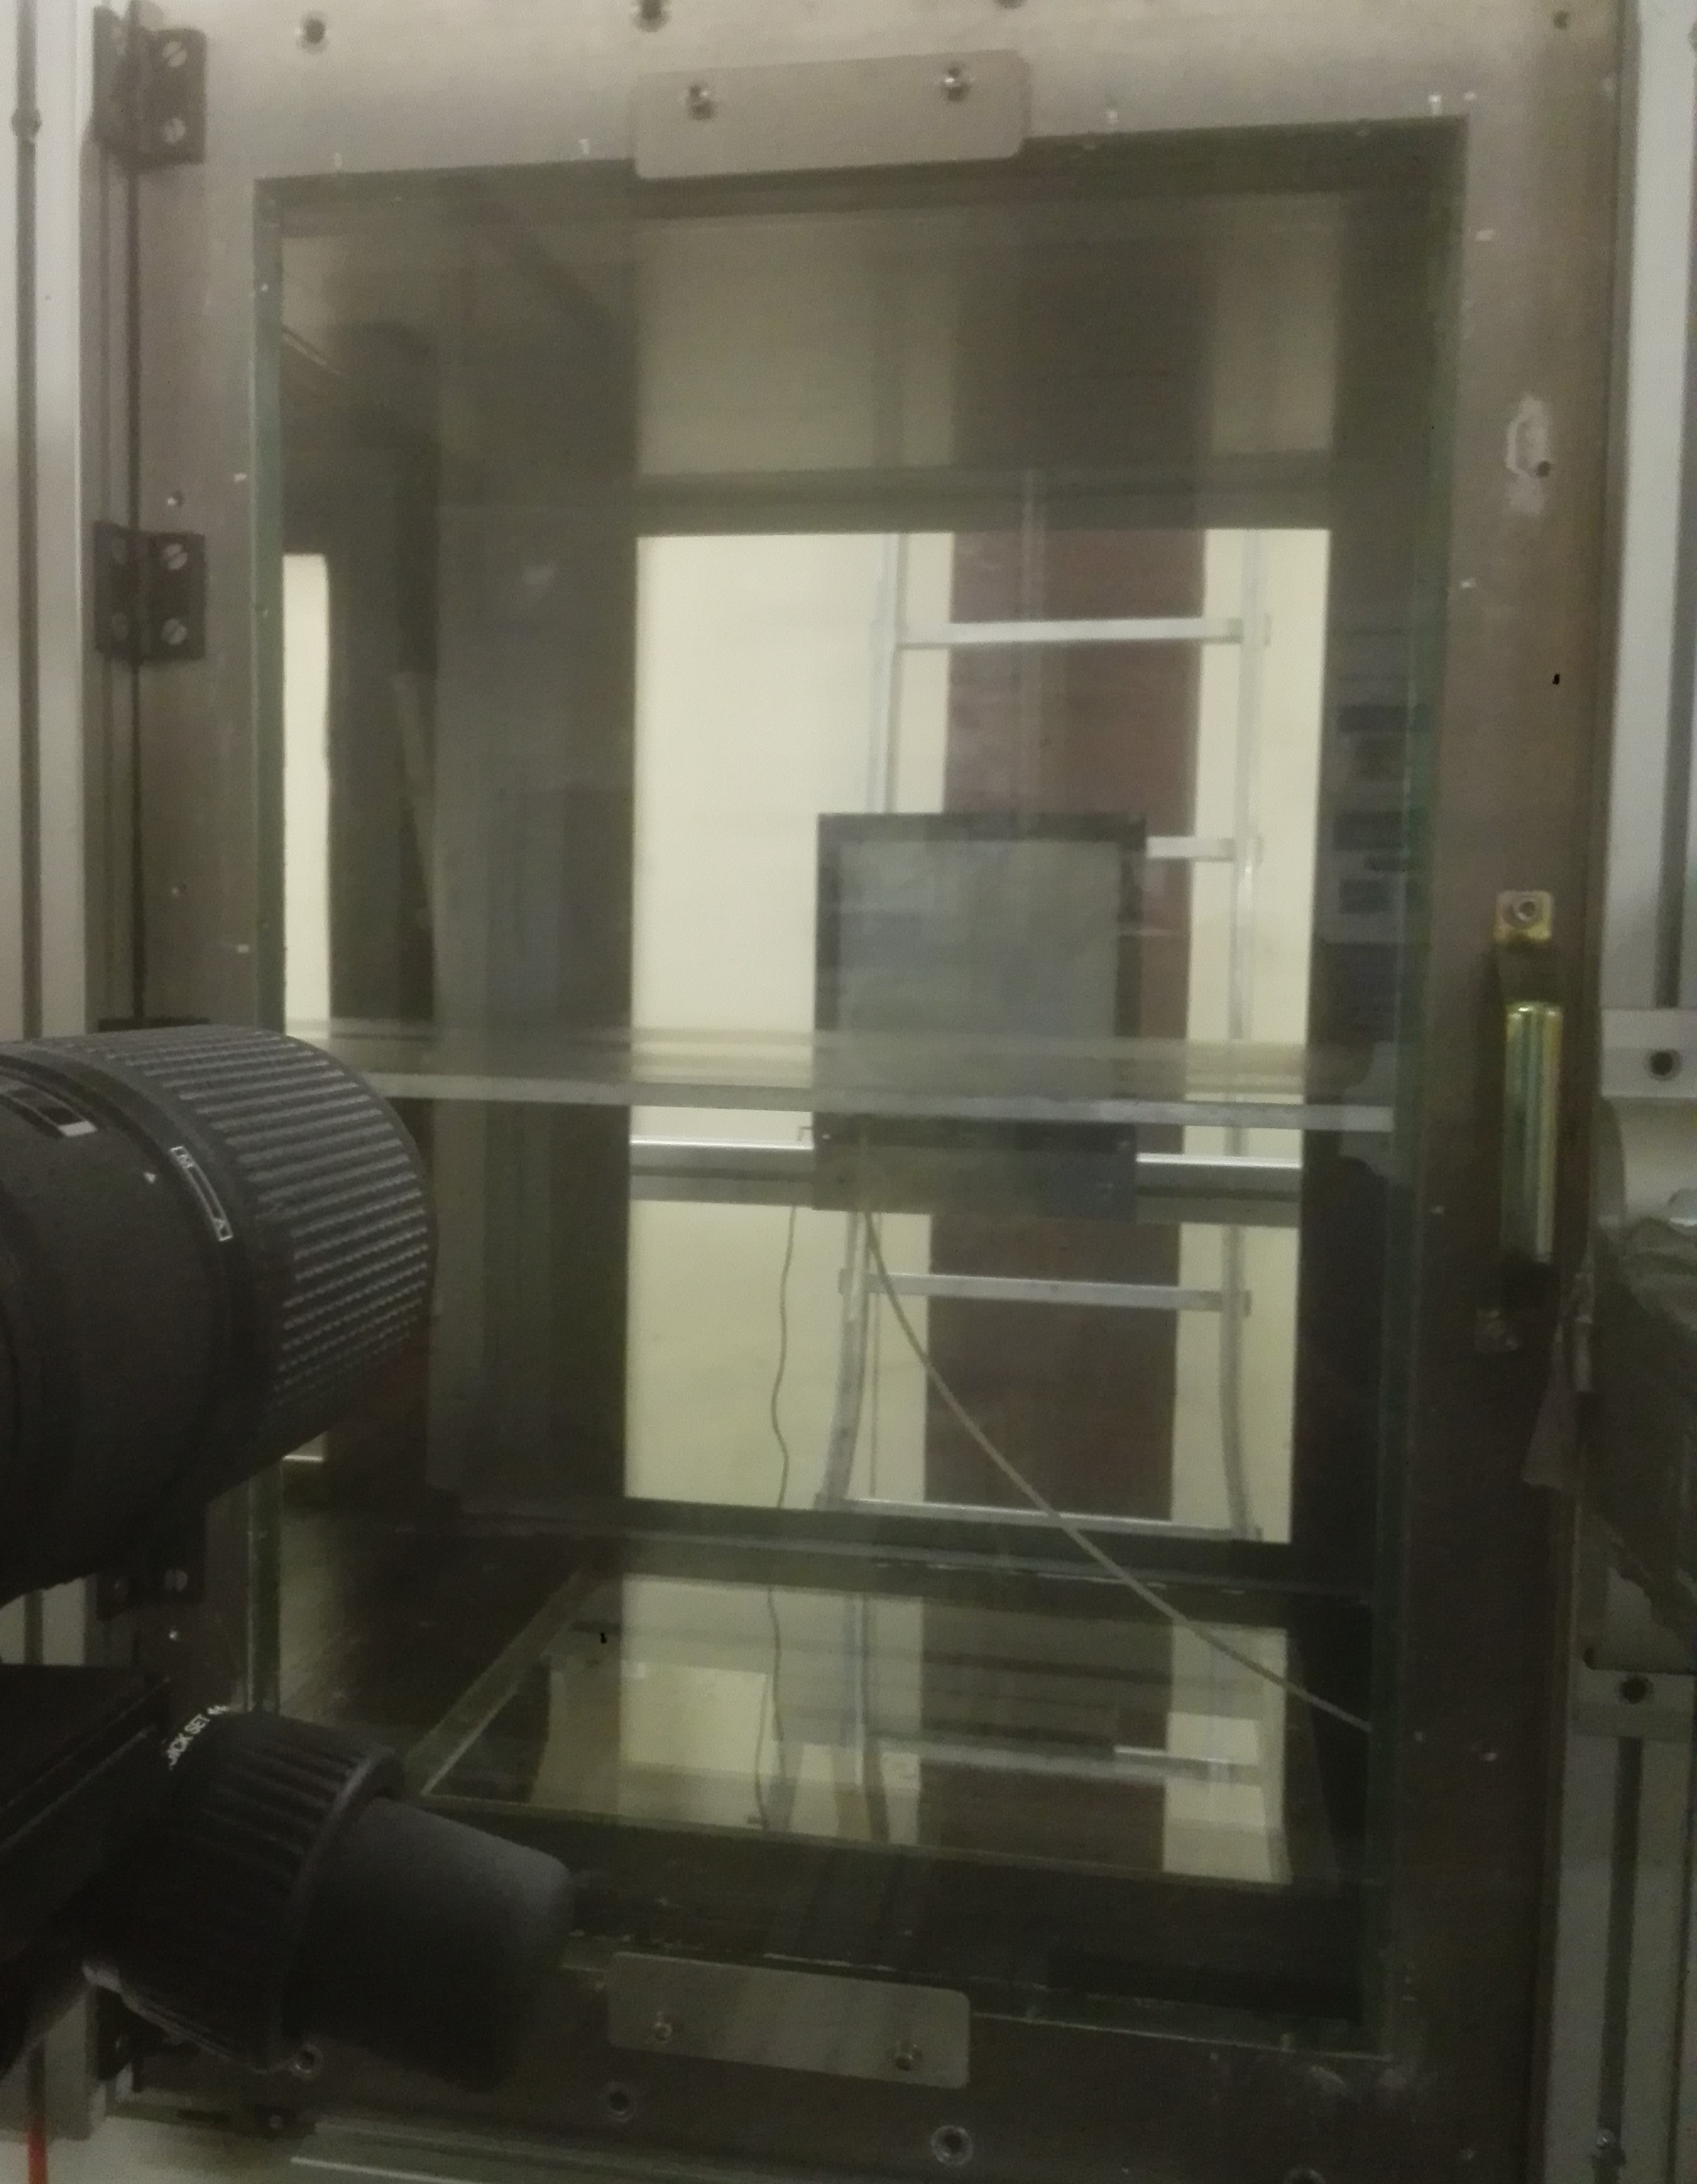
\includegraphics[width = 0.4\linewidth]{./image/Surface.jpg}
	\caption{Camera, surface et écran à laser}
	\label{fig:Plan}
\end{figure}
\begin{figure}[ht]
\centering
	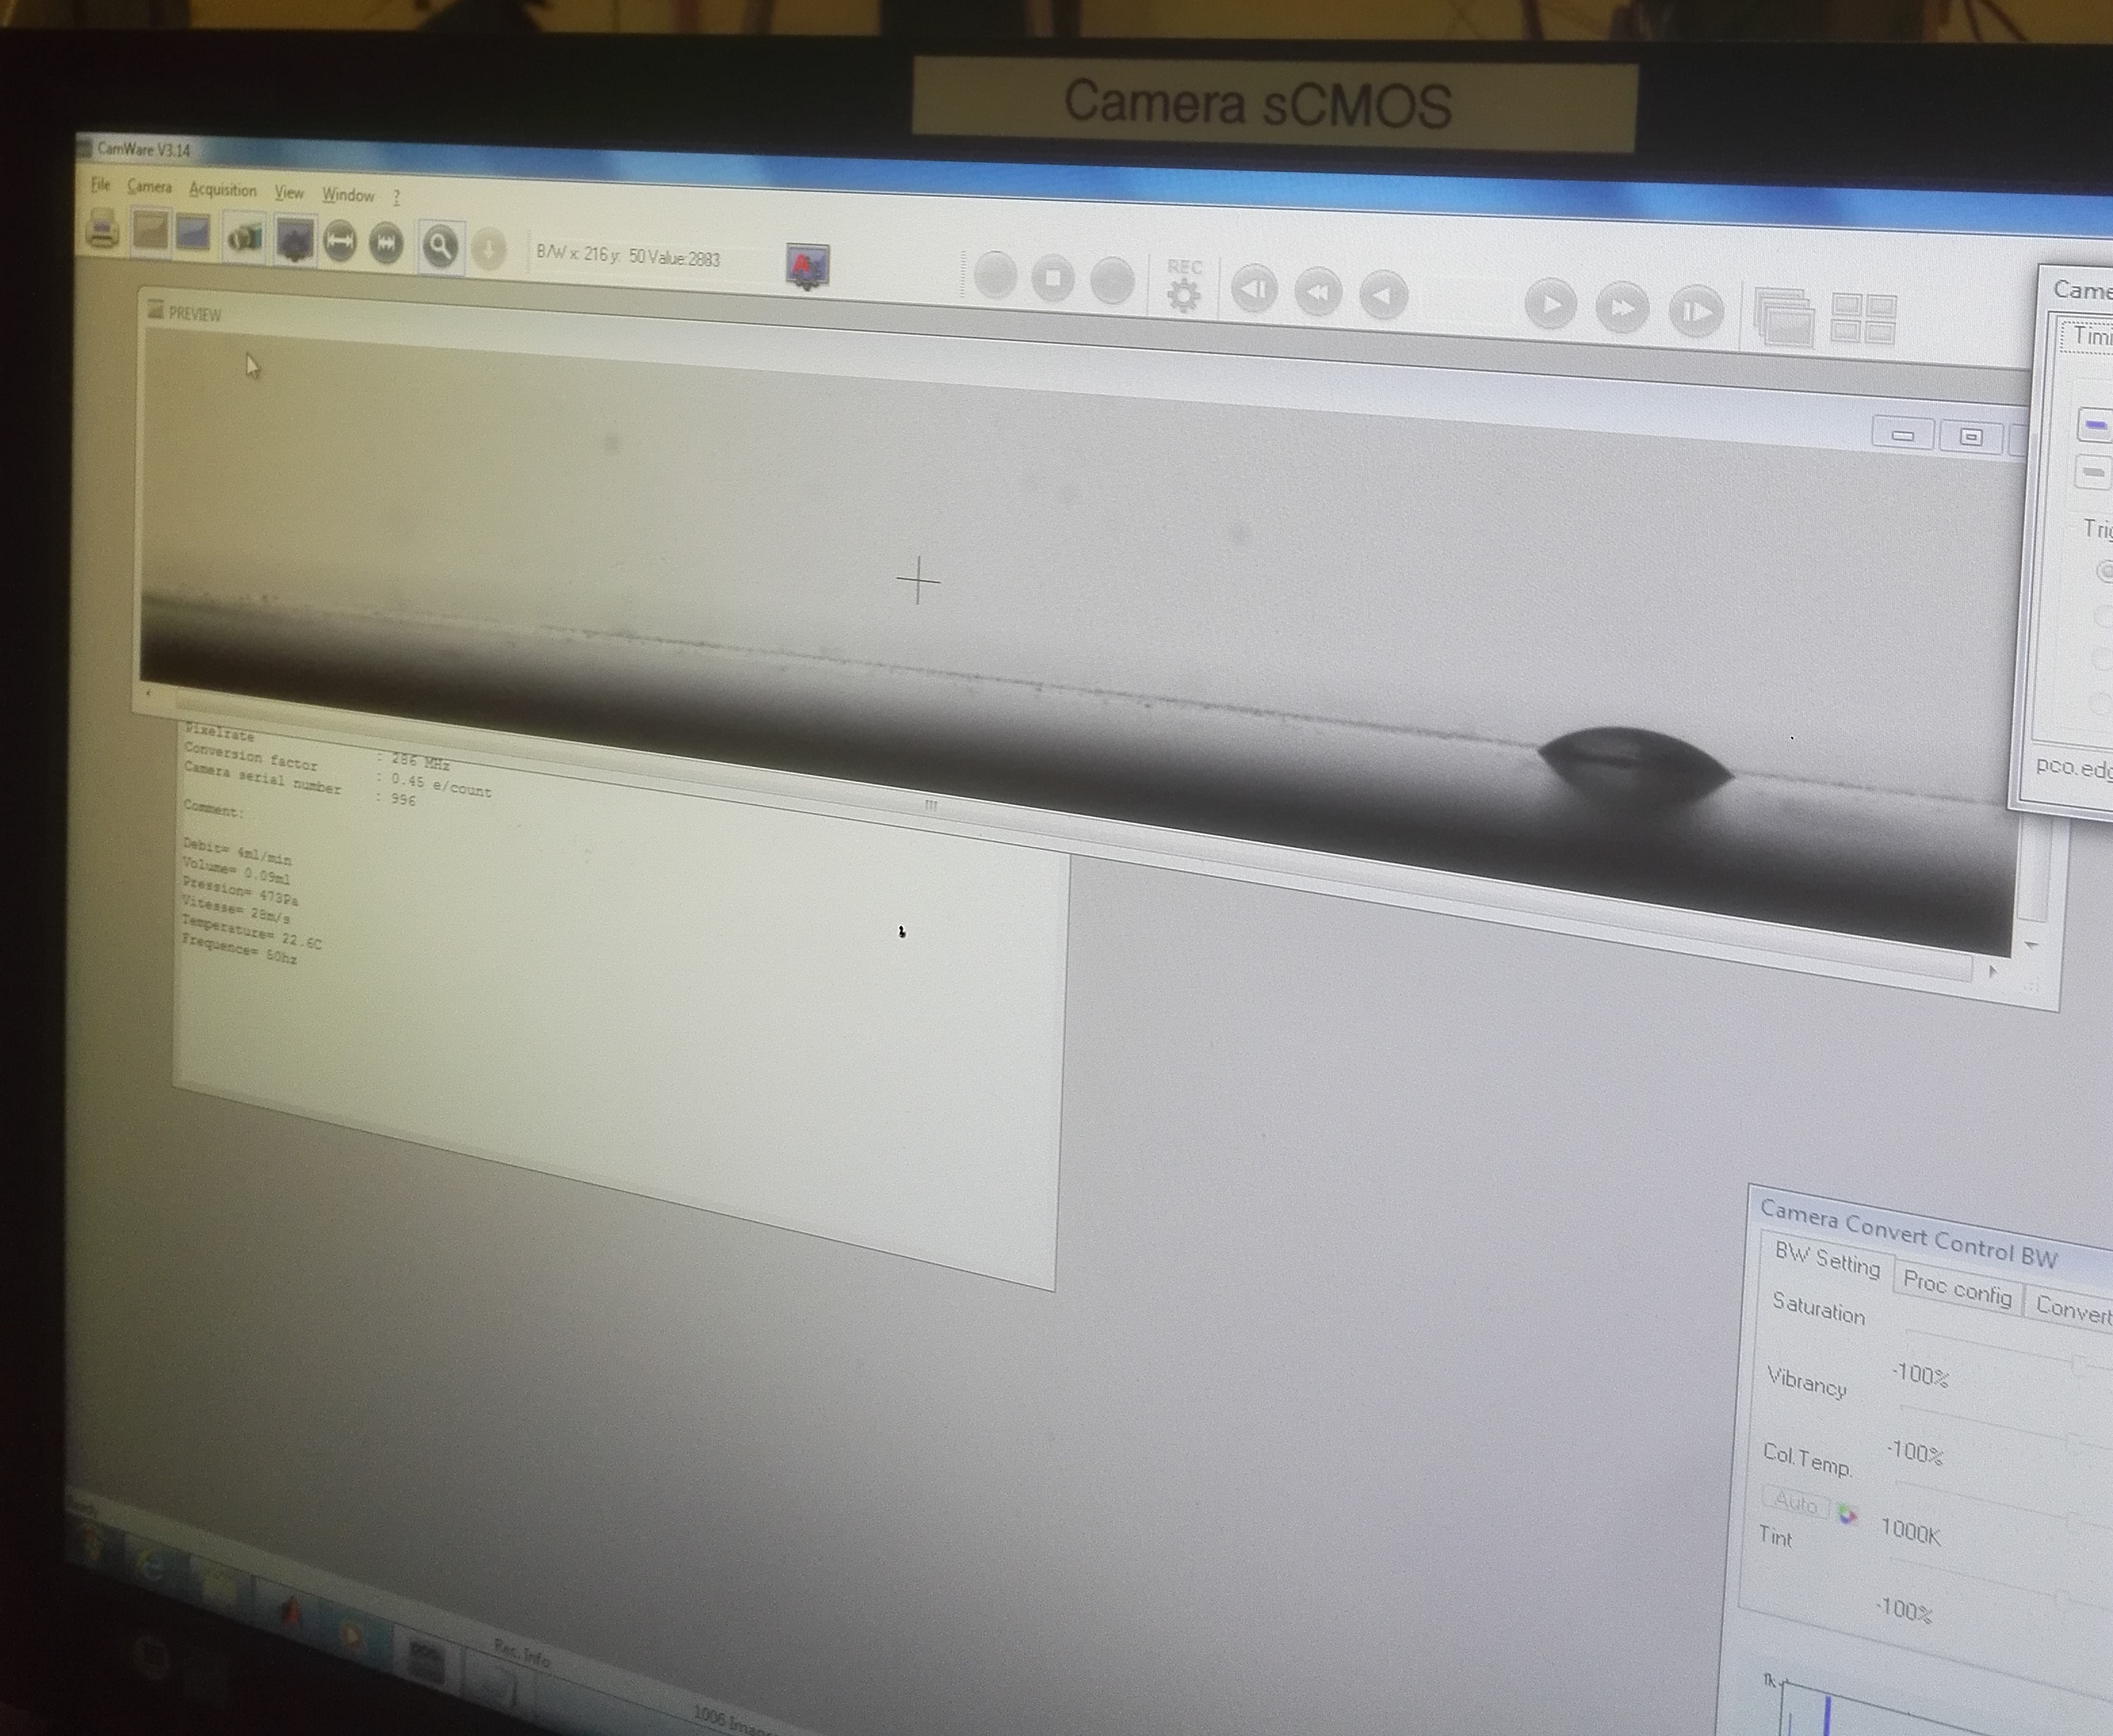
\includegraphics[width = 0.5\linewidth]{./image/Ecran.jpg}
	\caption{Ecran}
	\label{fig:Ecran d'observation}
\end{figure}

\newpage

\section{Anémomètre à fil chaud}
C'est l'anémomètre à fil chaud qui nous a permis de déterminer les profils de la couche limite dans notre écoulement.

Le principe de l'anénomètre à fil chaud est de placer un fil chaud (de l'ordre de $1mm$ de long et de $1\mu m$ de diamètre) dans l'écoulement et de maintenir sa température constante.

l'écoulement retirera une énergie au fil chaud et pour maintenir la température constante du fil chaud, on lui fournit une certaine énergie et cette énergie fournie (la tension qu'il a fallu fournir) est liée à la vitesse au niveau du fil chaud.


\section{Paramètres mesurés}

\begin{figure}[ht]
	\centering
	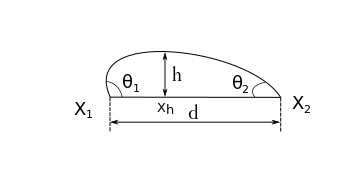
\includegraphics[scale = 1]{./image/rrgou2.png}
	\caption{Paramètres mesurés}
\end{figure}

\begin{figure}[hb]
	\centering
	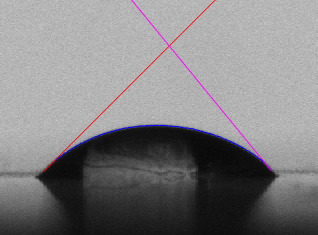
\includegraphics[scale = 0.6]{./image/crop_tvitesse=28_volume=003.png}
	\caption{Goutte d'eau de volume $0.03$ml avec $\theta_{a} = 45^{o}$ et $\theta_{r} = 50.17^{o}$}
\end{figure}


\end{document}
